\begin {document}

\title {\ZHH \huge UML类图关系整理}
\author {\small gaccob}
\date {\small 2013 年 10 月 1 日}
\maketitle
\begin {center}
{\ZHH \small 标签: UML, 类图}
\end {center}

\vspace {10pt}
\section {\ZHH UML关系图一览} {
    \begin {figure} [htbp]
        \centering
        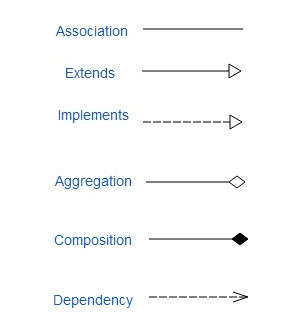
\includegraphics [width=180pt, keepaspectratio] {relation.png}
    \end {figure}
}

\section {\ZHH Association 关联} {
    \begin {itemize}
    \item {双向关联: 双方都知道对方的存在, 可以调用对方的public属性和方法.}
    \item {单向关联: A知道B, 可以调用B的public属性和方法, 但是没有生命期的依赖. }
    \item {自身关联: 自己引用自己. }
    \begin {figure} [htbp]
        \centering
        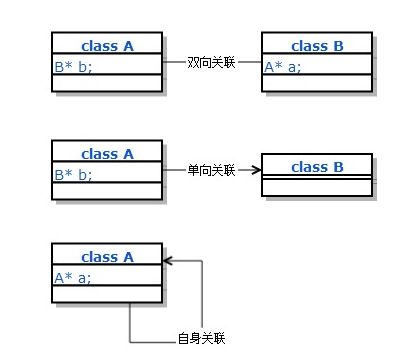
\includegraphics [width=280pt, keepaspectratio] {association.png}
    \end {figure}
    \end {itemize}
}

\section {\ZHH Extends/Implementation 继承/实现} {
    { 没有叫做泛化, 是因为一直觉得这个词太学术了…… 个人觉得这两个在C++中没有太大的区别, 如果是继承自纯虚基类, 也许用implementation更好一些. } \\
    \begin {figure} [htbp]
        \centering
        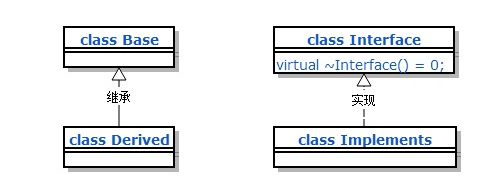
\includegraphics [width=320pt, keepaspectratio] {implementation.png}
    \end {figure}
}

\section {\ZHH Aggregation/Composition 聚合/组合} {
    { 简单的来说: A和a有整体-部分关系时, 如果A负责a的生命周期, 则叫组合; 如果A不管a的生命周期, 则叫聚合. } \\
    \begin {figure} [htbp]
        \centering
        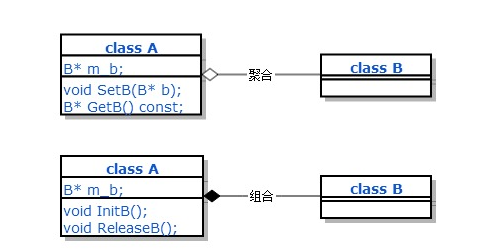
\includegraphics [width=320pt, keepaspectratio] {aggregation.png}
    \end {figure}
}

\section {\ZHH Dependency 依赖} {
    { A需要用到B的时候, A就依赖于B, 最常见的例子是A的某个函数参数是B的对象. } { \textcolor {blue} {应该避免相互依赖.} } \\
    \begin {figure} [htbp]
        \centering
        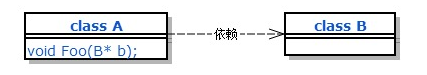
\includegraphics [width=280pt, keepaspectratio] {dependency.png}
    \end {figure}
}

\section {\ZHH 参考文档} {
    \begin {enumerate}
    \item {\href{http://www.cnblogs.com/riky/archive/2007/04/07/704298.html}{UML关系类图大全} }
    \item {\href{http://blog.csdn.net/dylgsy/article/details/1076044}{UML类图关系全面剖析} }
    \end {enumerate}
}

\end {document}
